\makeatletter
\def\input@path{{../}}
\makeatother

\documentclass[/main.tex]{subfiles}
\graphicspath{{./pics/}{appAllResults/pics/}}

\newcommand{\allmodeplots}[3]{% inputs are file name modifier, description of mode, and discription of gamma
  \FloatBarrier
  \begin{sidewaystable}[p]
    \caption[#3 of #2: Energy systematics table]{ \label{tab:energysystematics}
      Table of energy estimation uncertainties for the #3.
    }
    \resizebox{\textwidth}{!}{%
      \input{appBlindResults/tables/table_#1_pseff.tex} }
  \end{sidewaystable}
  
  \begin{figure}[!htb]
    \centering
    \subfloat[Simulated BG Sum Energy Spectrum]{\includegraphics[width=.5\linewidth]{BGSumECuts_#1}}
    \subfloat[Simulated ES Sum Energy Spectrum]{\includegraphics[width=.5\linewidth]{ESSumECuts_#1}}\\
    \subfloat[Simulated BG Coincident Energy Spectrum]{\includegraphics[width=.5\linewidth]{BGCoinECuts_#1}}
    \subfloat[Simulated ES Coincident Energy Spectrum]{\includegraphics[width=.5\linewidth]{ESCoinECuts_#1}}
    \caption[#3 of #2: Sum and coincident simulated energy spectra with cuts]{
      Sum energy and coincident energy spectra for the #3.
    }
  \end{figure}
  
  \begin{figure}[p]
    \centering
    \subfloat[Simulation]{\includegraphics[width=0.7\linewidth]{BG2Dcuts_#1}}\\
    \subfloat[Data]{\includegraphics[width=0.7\linewidth]{Data2Dcuts_#1}}
    \caption[#3 of #2: 2D plots of sum and coincident energy cuts in simulations and data]{
      Simulated and measured multiplicity 2 energy spectrum with sum and coincident energy cuts included for the #3.
    }
  \end{figure}
  
  \begin{figure}[p]
    \centering
    \subfloat[Effect of all cuts on ROI]{\includegraphics[width=0.8\linewidth]{ESAllCuts_#1}}\\
    \subfloat[Table of efficiencies]{\input{tables/table_#1_efficiency.tex}}
    \caption[#3 of #2: Effect of all cuts in ROI]{Plot showing effect of cuts applied sequentially on ROI peak and table of detection efficiencies for the #3.}
  \end{figure}


  \begin{figure}[p]
    \centering
    \subfloat[Simulated BG Cuts]{\includegraphics[width=.5\linewidth]{BGAllCuts_#1}}
    \subfloat[Data Cuts]{\includegraphics[width=.5\linewidth]{DataAllCuts_#1}}\\
    \subfloat[Data ROIs]{\includegraphics[width=0.5\linewidth]{DataROIs_#1}}
    \caption[#3 of #2: Cuts appliled to simulated and measured background data]{
      Effect of all cuts applied to measured and simulated background data.
    }
  \end{figure}
  
  \begin{sidewaystable}[p]
    \centering
    \input{tables/table_#1_bgcuts.tex}
    \caption[#3 of #2: Summary of cut efficiency in BG and data]{
      Table of cut descriptions and efficiencies for simulated backgrounds and measured data for the #3.
    }
  \end{sidewaystable}
  \FloatBarrier
}

\begin{document}
\onlyinsubfile{\appendix}
\chapter{Detailed Results for All Decay Modes}

This appendix will present figures and tables detailing the simulations, cuts, efficiencies and results for each decay mode and peak, after unblinding.

\begin{figure}[!htb]
  \centering
  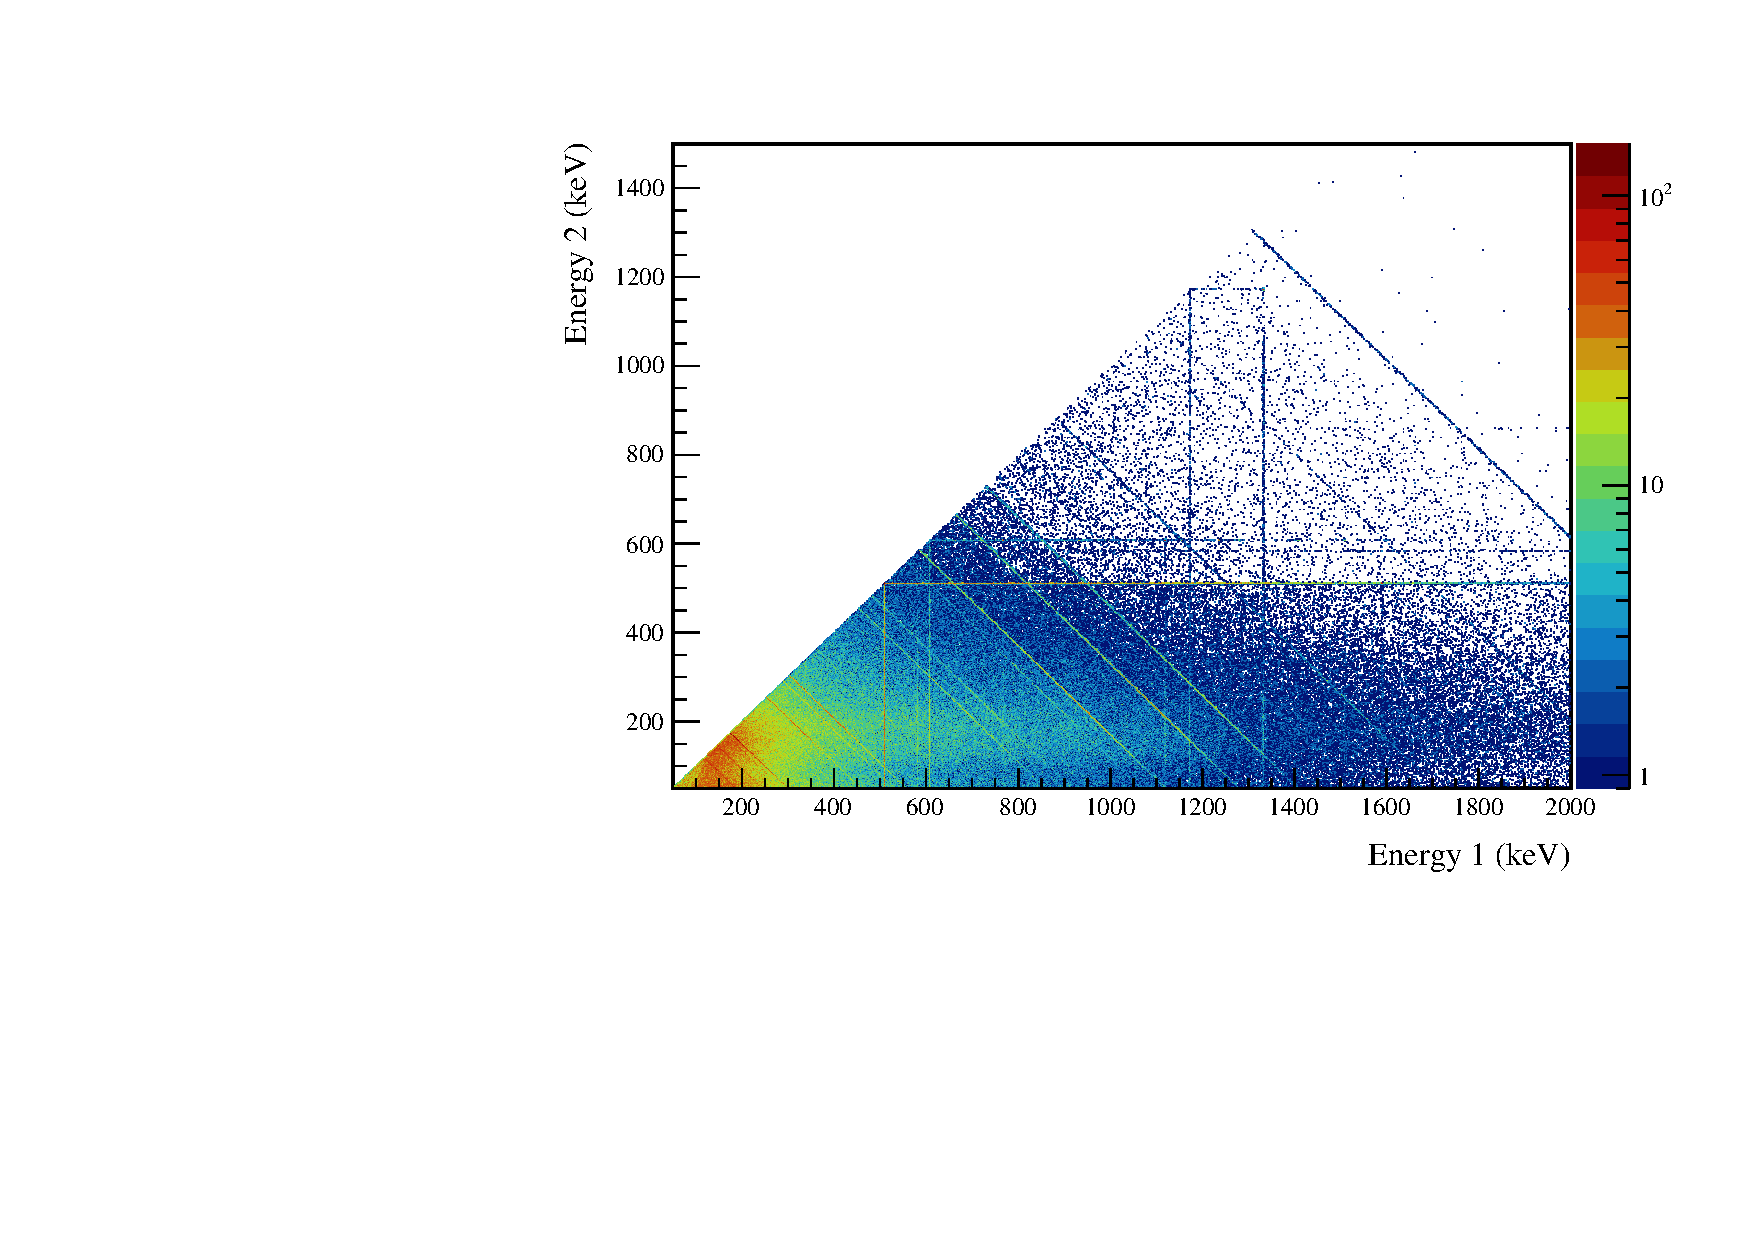
\includegraphics[width=.8\linewidth]{BGsim}
  \caption{
    Simulation using early version of background model.
    }
\end{figure}
\begin{figure}[!htb]
  \centering
  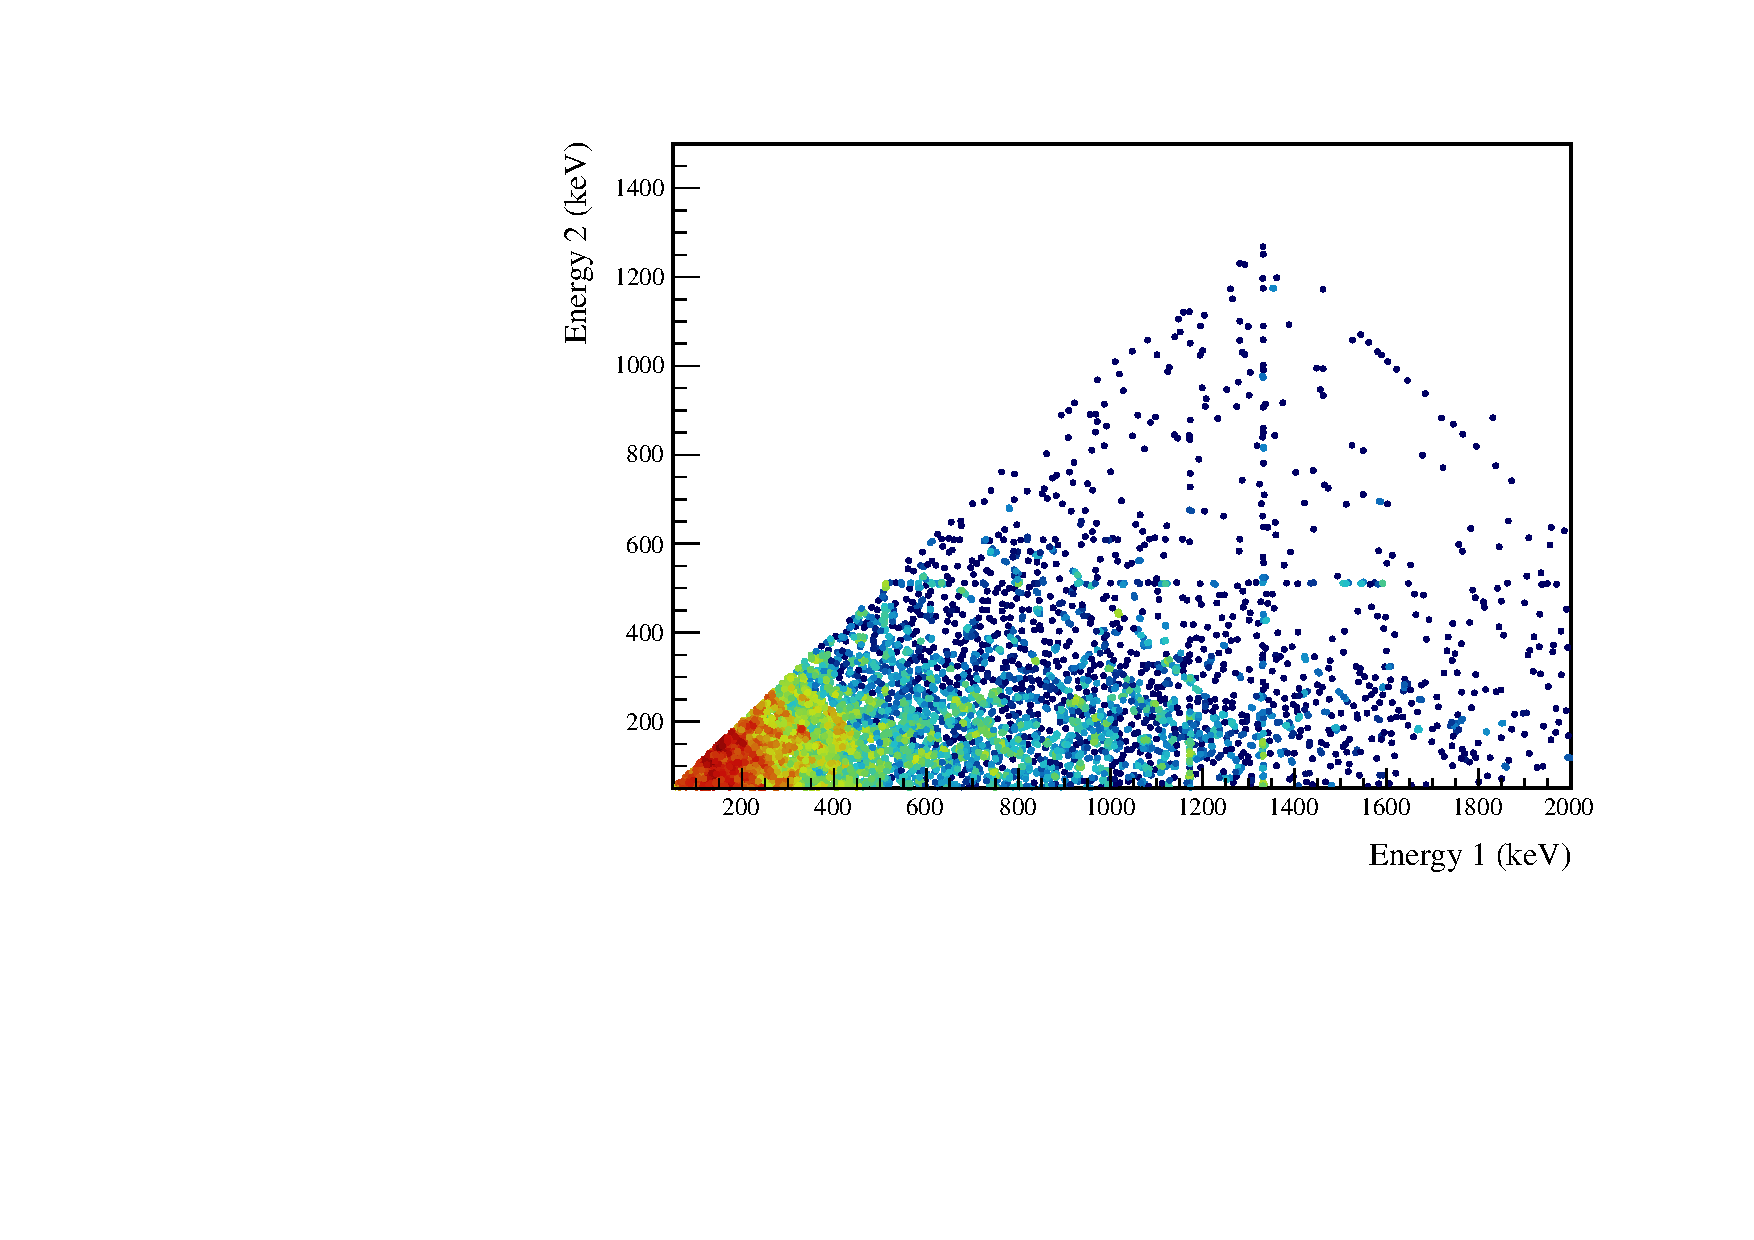
\includegraphics[width=.8\linewidth]{Data2D}
  \caption{
    All 2-detector events, colored using a Gaussian density kernel.
    }
\end{figure}

\begin{table}[!h]
  \scriptsize
  \centering
  \begin{tabular}{|c|c|c c c c c|c|c|}
\hline  Decay Mode & Peak & Module & $n_{ROI}$ & $m_{BG}$ & \makecell{Expected\\ROI BGs} & $T^*\,(\times 10^{23} \mathrm{y})$ & \makecell{$T_{1/2}\,(\times 10^{23} \mathrm{y})$ \\ 90\% Limit} & \makecell{$T_{1/2}\,(\times 10^{23} \mathrm{y})$ \\ 90\% Sensitivity} \\
\hline
\multirow{5}{*}{\decaySP{2}{0}{1}} & \multirow{2}{*}{559 keV} & M1 & 2 & 23 & 0.88 & $8.41 \pm 0.62$ & $>1.9$ & $>3.2$ \\
     &      & M2 & 0 & 2 & 0.09 & $2.10 \pm 0.41$ & $>1.5$ & $>1.5$ \\
     & \multirow{2}{*}{563 keV} & M1 & 0 & 23 & 0.97 & $8.42 \pm 0.62$ & $>6.2$ & $>3.2$ \\
     &      & M2 & 0 & 2 & 0.08 & $2.08 \pm 0.40$ & $>1.5$ & $>1.5$ \\
     & Combined &  &  &  &  &  & $>6.8$ & $>7.0$ \\
\hline\multirow{3}{*}{\decaySP{2}{2}{1}} & \multirow{2}{*}{559 keV} & M1 & 0 & 16 & 0.68 & $10.43 \pm 1.10$ & $>7.6$ & $>7.6$ \\
     &      & M2 & 0 & 1 & 0.04 & $2.66 \pm 0.98$ & $>1.8$ & $>1.8$ \\
     & Combined &  &  &  &  &  & $>9.6$ & $>5.3$ \\
\hline\multirow{7}{*}{\decaySP{2}{2}{2}} & \multirow{2}{*}{559 keV} & M1 & 2 & 38 & 1.46 & $7.24 \pm 0.97$ & $>1.8$ & $>2.9$ \\
     &      & M2 & 0 & 5 & 0.22 & $1.89 \pm 0.97$ & $>1.1$ & $>1.1$ \\
     & \multirow{2}{*}{657 keV} & M1 & 1 & 20 & 0.69 & $5.49 \pm 0.77$ & $>1.8$ & $>4.0$ \\
     &      & M2 & 0 & 3 & 0.10 & $1.50 \pm 0.84$ & $>0.8$ & $>0.8$ \\
     & \multirow{2}{*}{1216 keV} & M1 & 0 & 29 & 0.79 & $3.14 \pm 0.95$ & $>2.2$ & $>1.0$ \\
     &      & M2 & 0 & 4 & 0.14 & $0.77 \pm 1.07$ & $>1.5$ & $>1.5$ \\
     & Combined &  &  &  &  &  & $>5.6$ & $>5.3$ \\
\hline\multirow{5}{*}{\decaySP{0}{0}{1}} & \multirow{2}{*}{559 keV} & M1 & 0 & 2 & 0.09 & $11.47 \pm 0.99$ & $>8.4$ & $>8.4$ \\
     &      & M2 & 0 & 0 & 0.00 & $2.92 \pm 0.59$ & $>2.1$ & $>2.1$ \\
     & \multirow{2}{*}{563 keV} & M1 & 0 & 2 & 0.09 & $11.32 \pm 0.98$ & $>8.3$ & $>8.3$ \\
     &      & M2 & 0 & 0 & 0.00 & $2.86 \pm 0.58$ & $>2.1$ & $>2.1$ \\
     & Combined &  &  &  &  &  & $>21.1$ & $>21.1$ \\
\hline\multirow{3}{*}{\decaySP{0}{2}{1}} & \multirow{2}{*}{559 keV} & M1 & 0 & 0 & 0.00 & $12.04 \pm 1.35$ & $>8.8$ & $>8.8$ \\
     &      & M2 & 0 & 0 & 0.00 & $3.01 \pm 1.10$ & $>2.0$ & $>2.0$ \\
     & Combined &  &  &  &  &  & $>11.0$ & $>11.0$ \\
\hline\multirow{7}{*}{\decaySP{0}{2}{2}} & \multirow{2}{*}{559 keV} & M1 & 0 & 2 & 0.08 & $7.16 \pm 1.01$ & $>5.2$ & $>5.2$ \\

  \caption{Table of results. $n_{ROI}$ and $m_{BG}$ are the number of observed events, after all cuts, in the Signal ROI and BG counting regions, respectively. $T^*=\ln2 \frac{N_A}{m_{76}}\epsilon_kM_{iso}T_{live}$ is used to calculate the number of expected signal counts from a half-life: $\langle s_k\rangle = \frac{T^*}{T_{1/2}}$. Physically, it represents the half-life that is expected to produce one count, based on exposure and detection efficiency. Limits and sensitivities were computed using the Rolke Confidence Intervals, which are similar to Feldman-Cousins, but account for nuisance parameter uncertainties in detection efficiency and exposure.}
\end{table}
\FloatBarrier

\section{Exposure}

\scriptsize
\begin{longtabu}{|c|c c|c|c c|c c|c|}
  \hline
  DS & M1 Detector Mask & M2 Detector Mask & \makecell{Run Time\\(days)} & \makecell{M1 L.T.\\(days)} & M1 Eff. & \makecell{M2 L.T.\\(days)} & M2 Eff. & \makecell{Exposure\\(kg$\cdot$y)} \\
  \hline
\endfirsthead
  \hline
  DS & M1 Detector Mask & M2 Detector Mask & \makecell{Run Time\\(days)} & \makecell{M1 L.T.\\(days)} & M1 Eff. & \makecell{M2 L.T.\\(days)} & M2 Eff. & \makecell{Exposure\\(kg$\cdot$y)} \\
  \hline
\endhead
  \hline
  \multicolumn{9}{r}{\textit{Continued on the next page}} \\
  \caption{List of subdatasets}
\endfoot
  \hline
  \caption[List of subdatasets, livetimes, efficiency and exposure]{\label{tab:subdatasets}
    List of each subdataset with its livetime, detection efficiency measured for the \bbes to \SP{0}{+}{1} decay, and total isotopic exposure. Note the large variance in the detection efficiency.
  }
\endlastfoot
\begin{tabular}{|c|c c|c|c c|c c|c|}
  \hline
  DS & M1 Detector Mask & M2 Detector Mask & \makecell{Run Time\\(days)} & \makecell{M1 L.T.\\(days)} & M1 Eff. & \makecell{M2 L.T.\\(days)} & M2 Eff. & \makecell{Exposure\\(kg$\cdot$y)} \\
  \hline
  DS1 & 061a08001e0e1c00 & 0000000000000000 & 2.64 & 2.60 & 1.72\% & 0.00 & 0.00\% & 0.109 \\
  DS1 & 161a08341e0e1c00 & 0000000000000000 & 0.02 & 0.02 & 2.00\% & 0.00 & 0.00\% & 0.001 \\
  DS1 & 161a0c341e0e1c00 & 0000000000000000 & 4.51 & 4.48 & 1.94\% & 0.00 & 0.00\% & 0.188 \\
  DS1 & 161a0c361e0e1c00 & 0000000000000000 & 3.49 & 3.48 & 1.47\% & 0.00 & 0.00\% & 0.146 \\
  DS1 & 1e1a00001e0e1c00 & 0000000000000000 & 7.82 & 7.73 & 2.04\% & 0.00 & 0.00\% & 0.324 \\
  DS1 & 1e1a08001e0e1c00 & 0000000000000000 & 37.30 & 36.87 & 2.23\% & 0.00 & 0.00\% & 1.547 \\
  DS1 & 1e1a08041e0e1c00 & 0000000000000000 & 6.26 & 6.19 & 2.30\% & 0.00 & 0.00\% & 0.260 \\
  DS1 & 1e1a08141e0e1c00 & 0000000000000000 & 0.26 & 0.25 & 2.32\% & 0.00 & 0.00\% & 0.011 \\
  DS1 & 1e1a08301e0e1c00 & 0000000000000000 & 1.40 & 1.37 & 2.33\% & 0.00 & 0.00\% & 0.057 \\
  DS1 & 1e1a08341e0e1c00 & 0000000000000000 & 7.58 & 7.50 & 2.12\% & 0.00 & 0.00\% & 0.315 \\
  DS1 & 1e1a0c001e0e1c00 & 0000000000000000 & 2.83 & 2.78 & 2.25\% & 0.00 & 0.00\% & 0.117 \\
  DS1 & 1e1a0c041e0e1c00 & 0000000000000000 & 0.04 & 0.04 & 2.24\% & 0.00 & 0.00\% & 0.002 \\
  DS1 & 1e1a0c341e0e1c00 & 0000000000000000 & 0.67 & 0.67 & 2.32\% & 0.00 & 0.00\% & 0.028 \\
  DS2 & 1e1a08001e0e1c00 & 0000000000000000 & 38.92 & 38.52 & 2.28\% & 0.00 & 0.00\% & 1.617 \\
  DS2 & 1e1a0c001e0e1c00 & 0000000000000000 & 1.22 & 1.19 & 2.27\% & 0.00 & 0.00\% & 0.050 \\
  DS3 & 1e1a0c3e1e0e1c00 & 0000000000000000 & 29.88 & 29.67 & 2.64\% & 0.00 & 0.00\% & 1.245 \\
  DS4 & 0000000000000000 & 1c061a16060e1e00 & 19.15 & 0.00 & 0.00\% & 18.85 & 1.89\% & 0.622 \\
  DS5a & 08000020040e1c00 & 18060a02040e1e00 & 1.49 & 1.48 & 0.72\% & 1.46 & 1.16\% & 0.110 \\
  DS5a & 08080020040e1c00 & 18060a16060e1e00 & 2.51 & 2.49 & 0.86\% & 2.47 & 1.56\% & 0.186 \\
  DS5a & 08080030040e1c00 & 18060a02040e1e00 & 0.01 & 0.01 & 0.91\% & 0.01 & 1.14\% & 0.001 \\
  DS5a & 0e1a04321e0e1c00 & 08020a16060e1e00 & 2.69 & 2.71 & 2.33\% & 2.66 & 1.23\% & 0.201 \\
  DS5a & 0e1a0c321e0e1c00 & 0000000000000000 & 0.65 & 0.63 & 2.59\% & 0.00 & 0.00\% & 0.026 \\
  DS5a & 0e1a0c321e0e1c00 & 08060a16060e1e00 & 1.24 & 1.24 & 2.58\% & 1.21 & 1.52\% & 0.092 \\
  DS5a & 0e1a0c321e0e1c00 & 18060a02040e1e00 & 2.94 & 2.92 & 2.35\% & 2.89 & 1.15\% & 0.218 \\
  DS5a & 0e1a0c321e0e1c00 & 18060a1406061600 & 0.04 & 0.04 & 2.56\% & 0.04 & 0.95\% & 0.003 \\
  DS5a & 0e1a0c321e0e1c00 & 18060a1606060600 & 3.19 & 3.15 & 2.52\% & 3.16 & 0.82\% & 0.237 \\
  DS5a & 0e1a0c321e0e1c00 & 18060a16060e0600 & 3.30 & 3.28 & 2.53\% & 3.29 & 0.84\% & 0.246 \\
  DS5a & 0e1a0c3e1e0e1c00 & 1806020606081800 & 1.75 & 1.73 & 2.80\% & 1.73 & 0.76\% & 0.129 \\
  DS5a & 0e1a0c3e1e0e1c00 & 18060216060c1c00 & 6.84 & 6.77 & 2.80\% & 6.74 & 1.12\% & 0.507 \\
  DS5a & 0e1a0c3e1e0e1c00 & 18060216060e1e00 & 13.48 & 13.30 & 2.77\% & 13.27 & 1.26\% & 0.996 \\
  DS5a & 0e1a0c3e1e0e1c00 & 18060816060e1c00 & 0.05 & 0.05 & 2.59\% & 0.05 & 1.30\% & 0.004 \\
  DS5a & 0e1a0c3e1e0e1c00 & 18060a0606060c00 & 2.16 & 2.12 & 2.77\% & 2.12 & 1.02\% & 0.159 \\
  DS5a & 0e1a0c3e1e0e1c00 & 18060a16040e1e00 & 0.76 & 0.76 & 2.76\% & 0.74 & 1.29\% & 0.056 \\
  DS5a & 0e1a0c3e1e0e1c00 & 18060a1606060c00 & 0.25 & 0.25 & 2.78\% & 0.25 & 1.11\% & 0.019 \\
  DS5a & 0e1a0c3e1e0e1c00 & 18060a1606061800 & 1.88 & 1.86 & 2.78\% & 1.86 & 1.04\% & 0.140 \\
  DS5a & 0e1a0c3e1e0e1c00 & 18060a1606061c00 & 9.20 & 9.13 & 2.75\% & 9.06 & 1.41\% & 0.682 \\
  DS5a & 0e1a0c3e1e0e1c00 & 18060a16060c1c00 & 7.89 & 7.79 & 2.78\% & 7.79 & 1.41\% & 0.584 \\
  DS5a & 0e1a0c3e1e0e1c00 & 18060a16060e1c00 & 11.68 & 11.53 & 2.43\% & 11.51 & 1.42\% & 0.864 \\
  DS5a & 0e1a0c3e1e0e1c00 & 18060a16060e1e00 & 5.21 & 5.15 & 2.76\% & 5.13 & 1.56\% & 0.386 \\
  DS5a & 0e1a0c3e1e0e1c00 & 18061216060e1e00 & 2.39 & 2.37 & 2.77\% & 2.37 & 1.34\% & 0.178 \\
  DS5b & 1e1a0c3e1e0c1c00 & 18061216060e1e00 & 24.46 & 24.09 & 2.75\% & 24.06 & 1.34\% & 1.805 \\
  DS5b & 1e1a0c3e1e0c1c00 & 18061a16060e1e00 & 0.75 & 0.75 & 2.75\% & 0.75 & 1.73\% & 0.056 \\
  DS5b & 1e1a0c3e1e0e1c00 & 18061216060e1e00 & 14.28 & 14.12 & 2.86\% & 14.07 & 1.24\% & 1.057 \\
  DS5c & 1e1a0c3e1e0c1c00 & 0000000000000000 & 0.67 & 0.67 & 2.65\% & 0.00 & 0.00\% & 0.028 \\
  DS5c & 1e1a0c3e1e0c1c00 & 00060216060e0e00 & 0.78 & 0.76 & 2.65\% & 0.78 & 0.84\% & 0.058 \\
  DS5c & 1e1a0c3e1e0c1c00 & 00060a16060e0e00 & 5.91 & 5.82 & 2.75\% & 5.83 & 1.07\% & 0.437 \\
  DS5c & 1e1a0c3e1e0c1c00 & 00061216060e0e00 & 38.85 & 38.45 & 2.73\% & 38.29 & 0.91\% & 2.877 \\
  DS6a & 12000000000c0800 & 1002020006040e00 & 4.94 & 4.89 & 0.16\% & 4.89 & 0.42\% & 0.366 \\
  DS6a & 12000c20000c1c00 & 18061216060c1e00 & 17.22 & 17.03 & 0.78\% & 17.03 & 1.13\% & 1.277 \\
  DS6a & 12020000040c0800 & 1802020006040e00 & 5.69 & 5.63 & 0.29\% & 5.62 & 0.50\% & 0.422 \\
  DS6a & 12020c00040c1800 & 1802020006040e00 & 7.90 & 7.79 & 0.68\% & 7.78 & 0.50\% & 0.584 \\
  DS6a & 12080c20000c1c00 & 18061216060c1e00 & 12.23 & 12.11 & 0.96\% & 12.09 & 1.13\% & 0.907 \\
  DS6a & 12120c3e1c0c1c00 & 18061216060c1e00 & 0.56 & 0.54 & 1.90\% & 0.56 & 1.10\% & 0.041 \\
  DS6a & 16020c10040c1800 & 1806020006060e00 & 14.89 & 14.73 & 0.90\% & 14.68 & 0.69\% & 1.103 \\
  DS6a & 160a0c321c0c1c00 & 1806021006061e00 & 5.87 & 5.80 & 2.05\% & 5.80 & 0.89\% & 0.435 \\
  DS6a & 1e0a0c321c0c1c00 & 0000000000000000 & 0.23 & 0.23 & 2.31\% & 0.00 & 0.00\% & 0.010 \\
  DS6a & 1e0a0c321c0c1c00 & 1806020006040200 & 10.00 & 9.89 & 2.31\% & 9.89 & 0.27\% & 0.741 \\
  DS6a & 1e0a0c321c0c1c00 & 1806020006040600 & 7.43 & 7.35 & 2.31\% & 7.32 & 0.41\% & 0.550 \\
  DS6a & 1e0a0c321c0c1c00 & 1806020006041600 & 4.88 & 4.83 & 2.31\% & 4.81 & 0.48\% & 0.362 \\
  DS6a & 1e0a0c321c0c1c00 & 1806021006061e00 & 6.11 & 6.05 & 2.31\% & 6.04 & 0.89\% & 0.453 \\
  DS6a & 1e120c3e1c0c1c00 & 18061216060c1e00 & 2.12 & 2.11 & 2.39\% & 2.09 & 1.13\% & 0.157 \\
  DS6a & 1e1a0c321c0c1c00 & 1806020006060e00 & 5.56 & 5.51 & 2.49\% & 5.53 & 0.69\% & 0.414 \\
  DS6a & 1e1a0c321c0c1c00 & 1806021006040e00 & 16.87 & 16.69 & 2.49\% & 16.64 & 0.69\% & 1.250 \\
  DS6a & 1e1a0c321c0c1c00 & 1806021006041e00 & 11.93 & 11.81 & 2.49\% & 11.79 & 0.86\% & 0.885 \\
  DS6a & 1e1a0c321c0c1c00 & 1806021006060e00 & 2.56 & 2.55 & 2.49\% & 2.55 & 0.73\% & 0.191 \\
  DS6a & 1e1a0c3a1c0c1c00 & 1806020006040e00 & 8.66 & 8.59 & 2.60\% & 8.59 & 0.65\% & 0.644 \\
  DS6a & 1e1a0c3a1c0c1c00 & 1806021006040e00 & 7.93 & 7.84 & 2.60\% & 7.83 & 0.69\% & 0.588 \\
  DS6a & 1e1a0c3a1c0c1c00 & 1806021006041e00 & 1.24 & 1.23 & 2.60\% & 1.23 & 0.86\% & 0.092 \\
  DS6a & 1e1a0c3e1c0c1c00 & 0000000000000000 & 0.06 & 0.05 & 2.69\% & 0.00 & 0.00\% & 0.002 \\
  DS6a & 1e1a0c3e1c0c1c00 & 1806000006040e00 & 7.85 & 7.81 & 2.69\% & 7.54 & 0.61\% & 0.577 \\
  DS6a & 1e1a0c3e1c0c1c00 & 1806020006041e00 & 5.96 & 5.88 & 2.65\% & 5.89 & 0.81\% & 0.441 \\
  DS6a & 1e1a0c3e1c0c1c00 & 1806021006041e00 & 3.56 & 3.52 & 2.69\% & 3.52 & 0.86\% & 0.264 \\
  DS6a & 1e1a0c3e1c0c1c00 & 18060210060c1e00 & 15.72 & 15.56 & 2.69\% & 15.51 & 0.92\% & 1.165 \\
  DS6a & 1e1a0c3e1c0c1c00 & 1806021206041e00 & 10.09 & 9.95 & 2.69\% & 9.97 & 0.89\% & 0.747 \\
  DS6a & 1e1a0c3e1c0c1c00 & 18060214060c0e00 & 5.65 & 5.60 & 2.69\% & 5.66 & 0.80\% & 0.422 \\
  DS6a & 1e1a0c3e1c0c1c00 & 18060214060c1e00 & 7.83 & 7.76 & 2.69\% & 7.74 & 0.98\% & 0.581 \\
  DS6a & 1e1a0c3e1c0c1c00 & 18060214060e1e00 & 58.28 & 57.56 & 2.67\% & 57.43 & 0.95\% & 4.311 \\
  DS6a & 1e1a0c3e1c0c1c00 & 1806121206041e00 & 1.00 & 0.98 & 2.69\% & 1.00 & 1.01\% & 0.074 \\
  DS6a & 1e1a0c3e1c0c1c00 & 18061212060c1e00 & 12.96 & 12.80 & 2.69\% & 12.80 & 1.07\% & 0.959 \\
  DS6a & 1e1a0c3e1c0c1c00 & 18061216060c1e00 & 26.05 & 25.76 & 2.69\% & 25.72 & 1.13\% & 1.930 \\
  \hline
  DSTotal & -- & -- & 621.97 & 615.24 & 2.35\% & 487.97 & 1.00\% & 41.923 \\
  \hline
\end{tabular}
\end{longtabu}
\normalsize

\begin{figure}
  \centering
  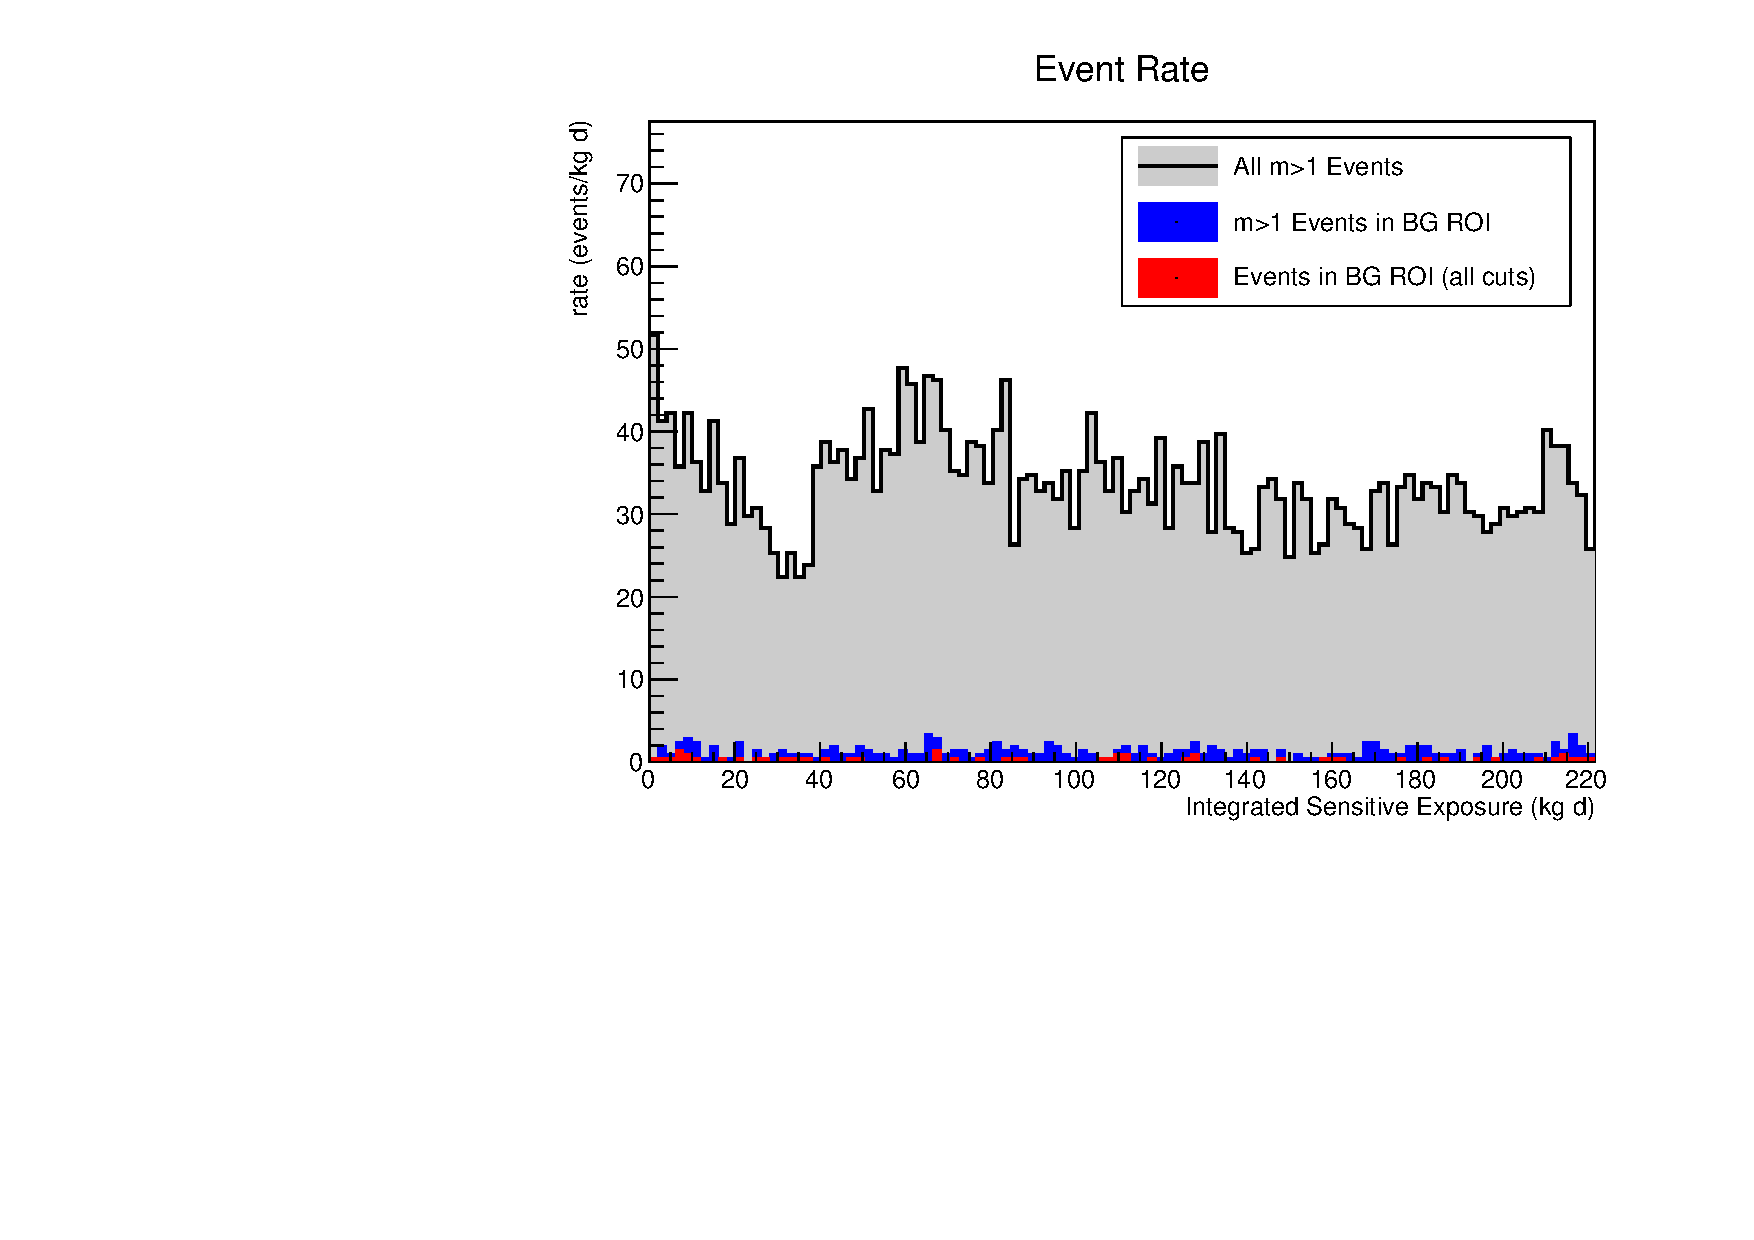
\includegraphics[width=.8\linewidth]{M1datarate}
  \caption{
    Module~1 Background rate vs sensitive exposure, defined as the detection efficiency for the \bbes to \SP{0}{+}{1} decay multiplied by the integrated exposure over all \Ge{76} in module~1.
    }
\end{figure}
\begin{figure}
  \centering
  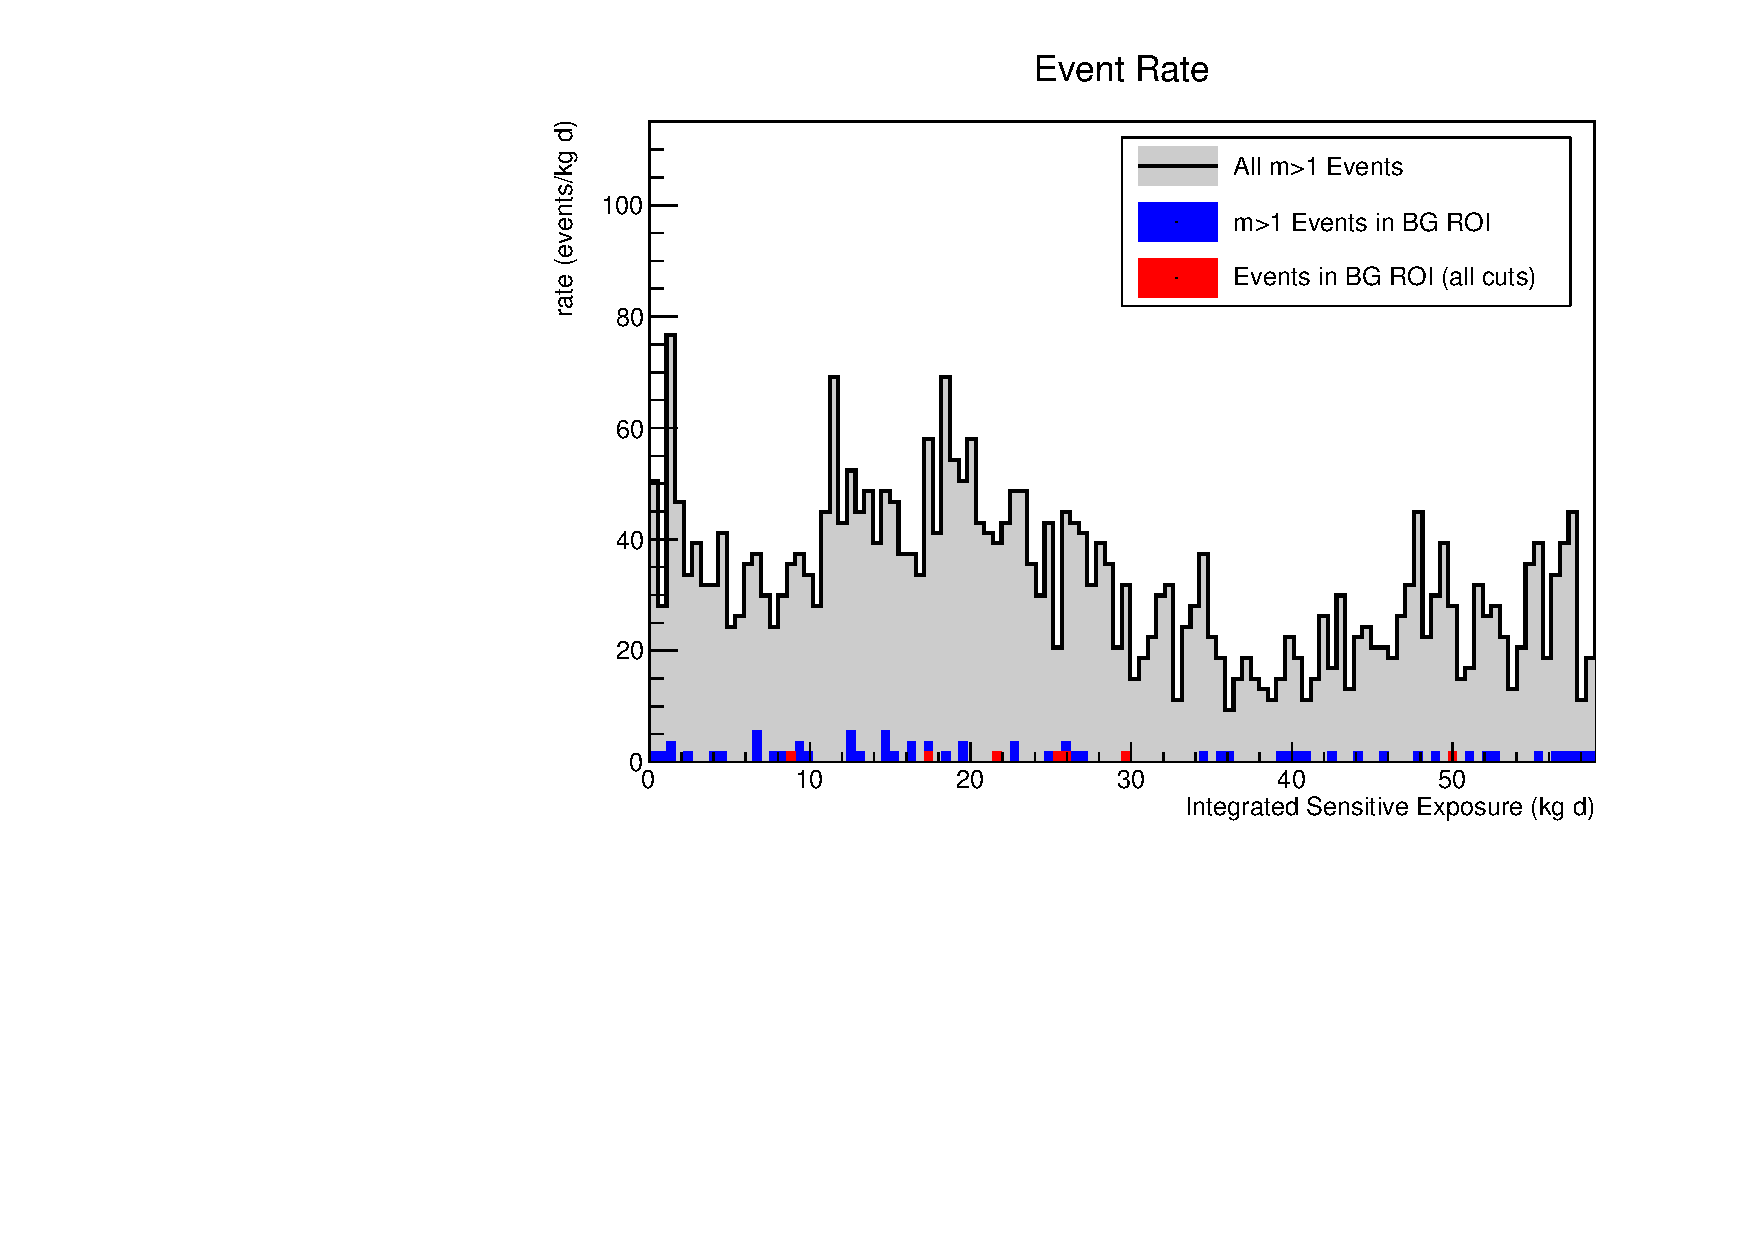
\includegraphics[width=.8\linewidth]{M2datarate}
  \caption{
    Module~2 Background rate vs sensitive exposure.
    }
\end{figure}

\section{\tnbb\ to \SP{0}{+}{1}}
Note that both the 559~and 563~keV peaks will be shown together since they use the same sets of cuts.
\begin{figure}[!htb]
  \centering
  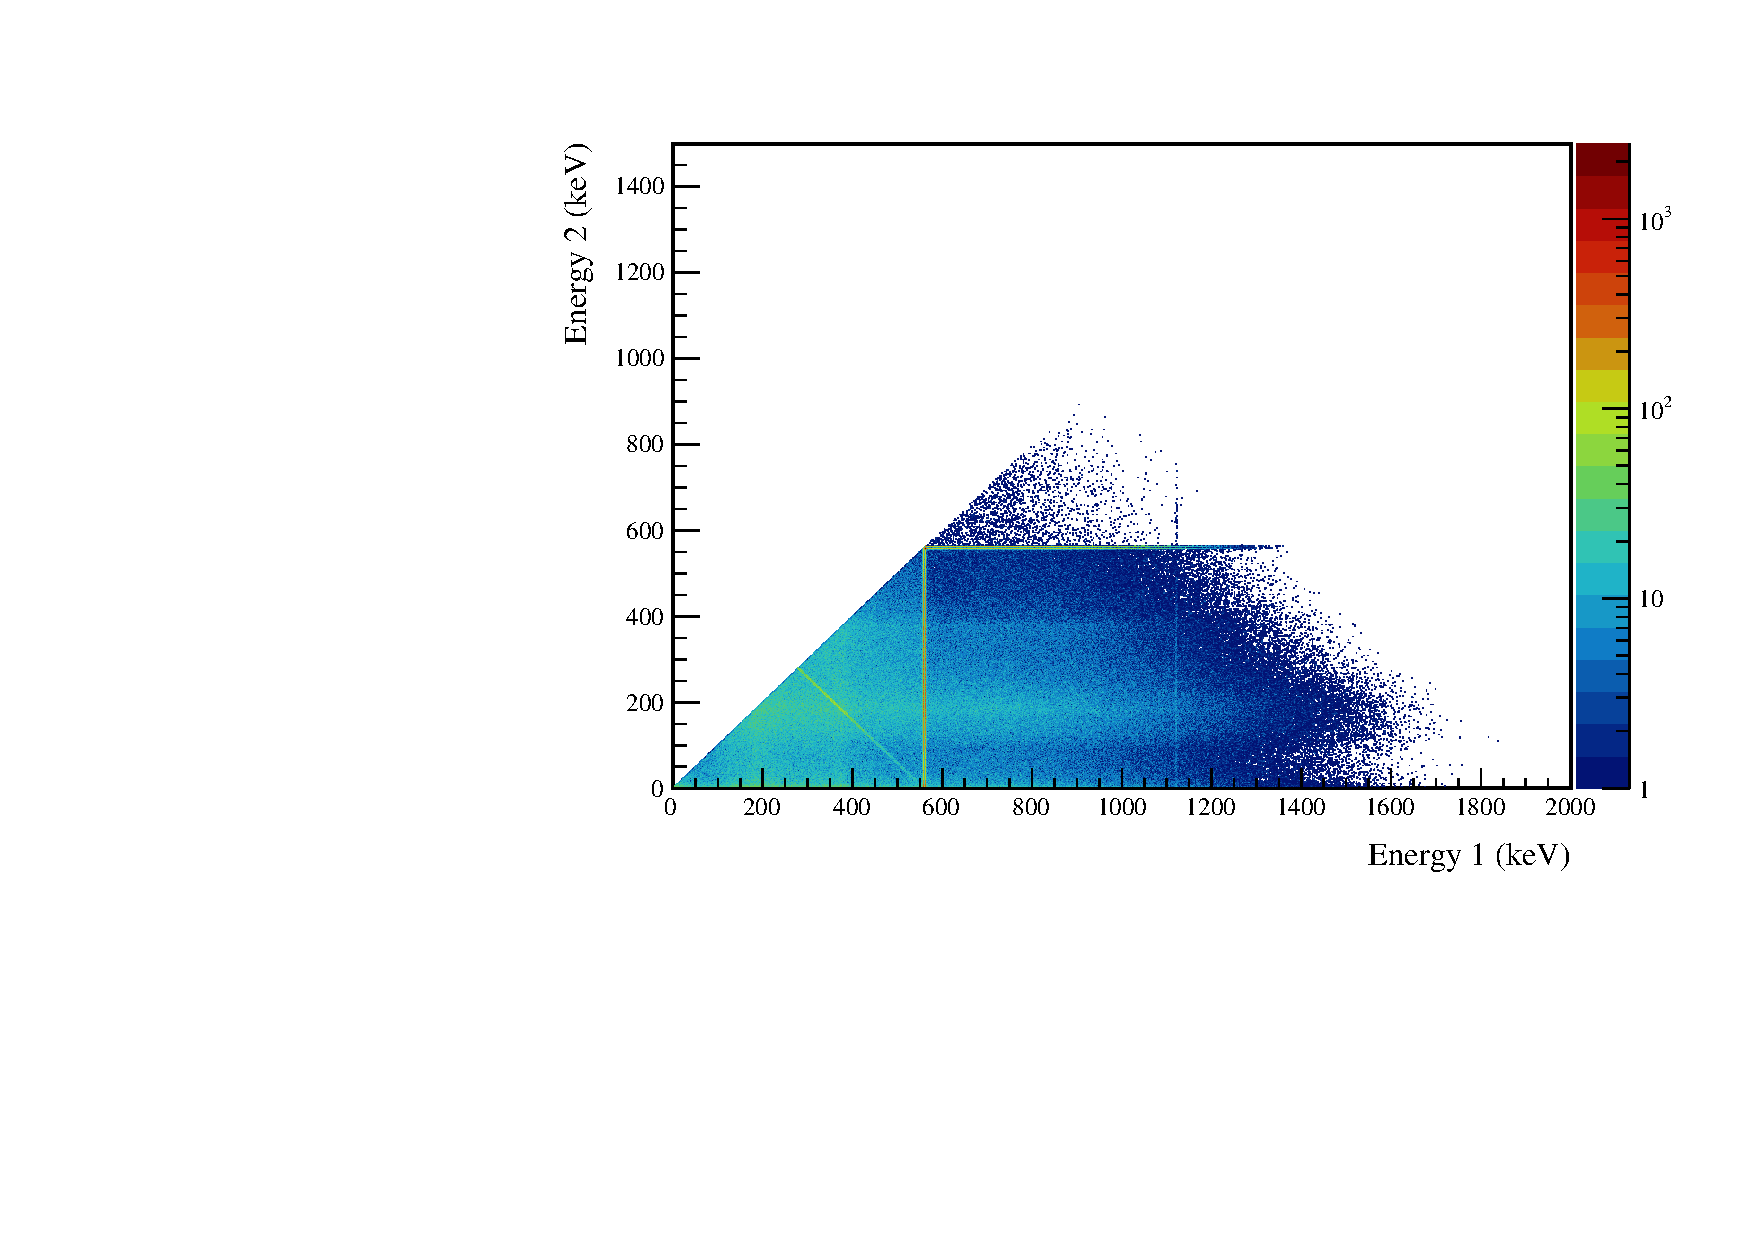
\includegraphics[width=.8\linewidth]{ESsim_2vBB_ES0_1}
  \caption[Simulation of \tnbb\ to \SP{0}{+}{1}]{
    Simulated multiplicity 2 energy spectrum of the \tnbb\ to \SP{0}{+}{1} decay mode}
\end{figure}

\allmodeplots{2vBB_ES0_1}{\tnbb\ to \SP{0}{+}{1}}{559~and 563~keV peaks}

\section{\tnbb\ to \SP{2}{+}{1}}
\begin{figure}[!htb]
  \centering
  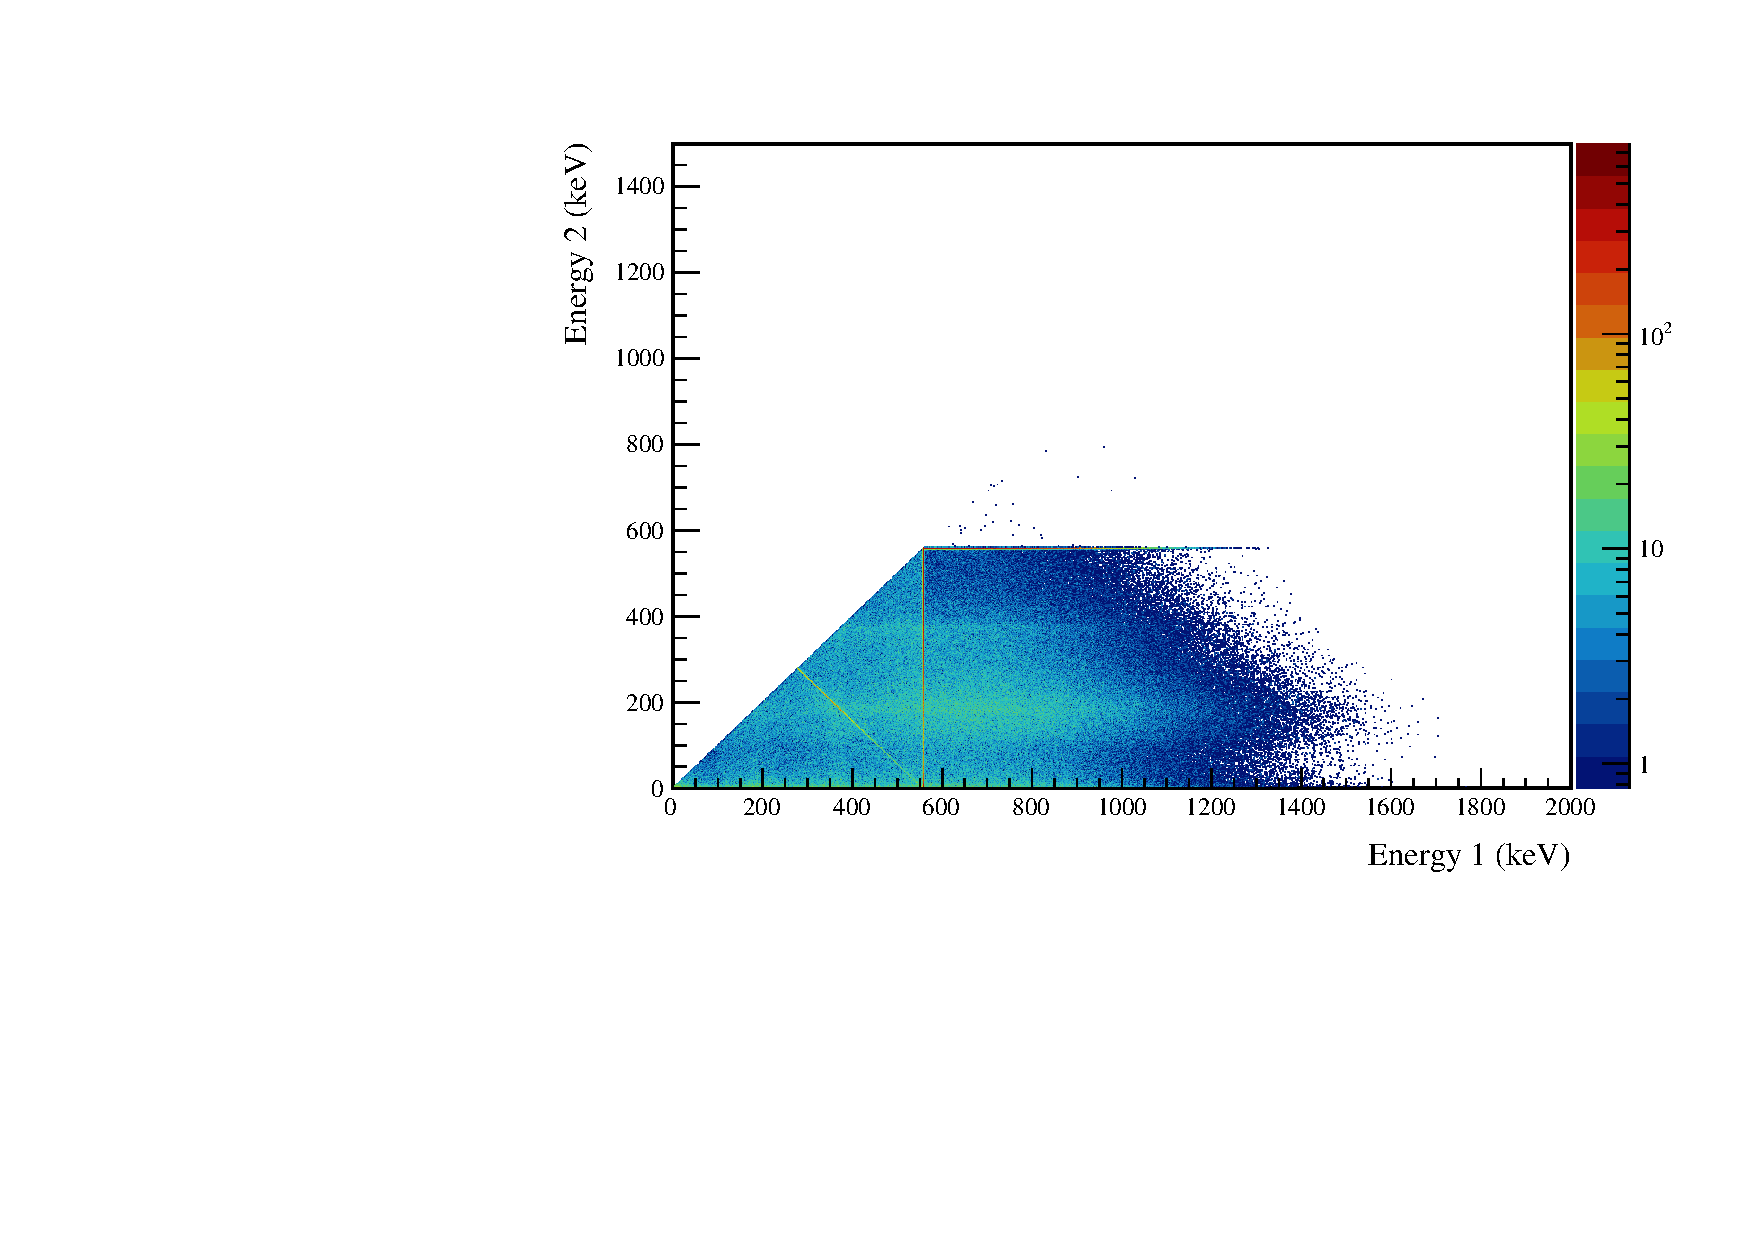
\includegraphics[width=.8\linewidth]{ESsim_2vBB_ES2_1}
  \caption[Simulation of \tnbb\ to \SP{2}{+}{1}]{
    Simulated multiplicity 2 energy spectrum of the \tnbb\ to \SP{2}{+}{1} decay mode}
\end{figure}

\allmodeplots{2vBB_ES2_1}{\tnbb\ to \SP{2}{+}{1}}{559~keV peak}

\section{\tnbb\ to \SP{2}{+}{2}}
\begin{figure}[!htb]
  \centering
  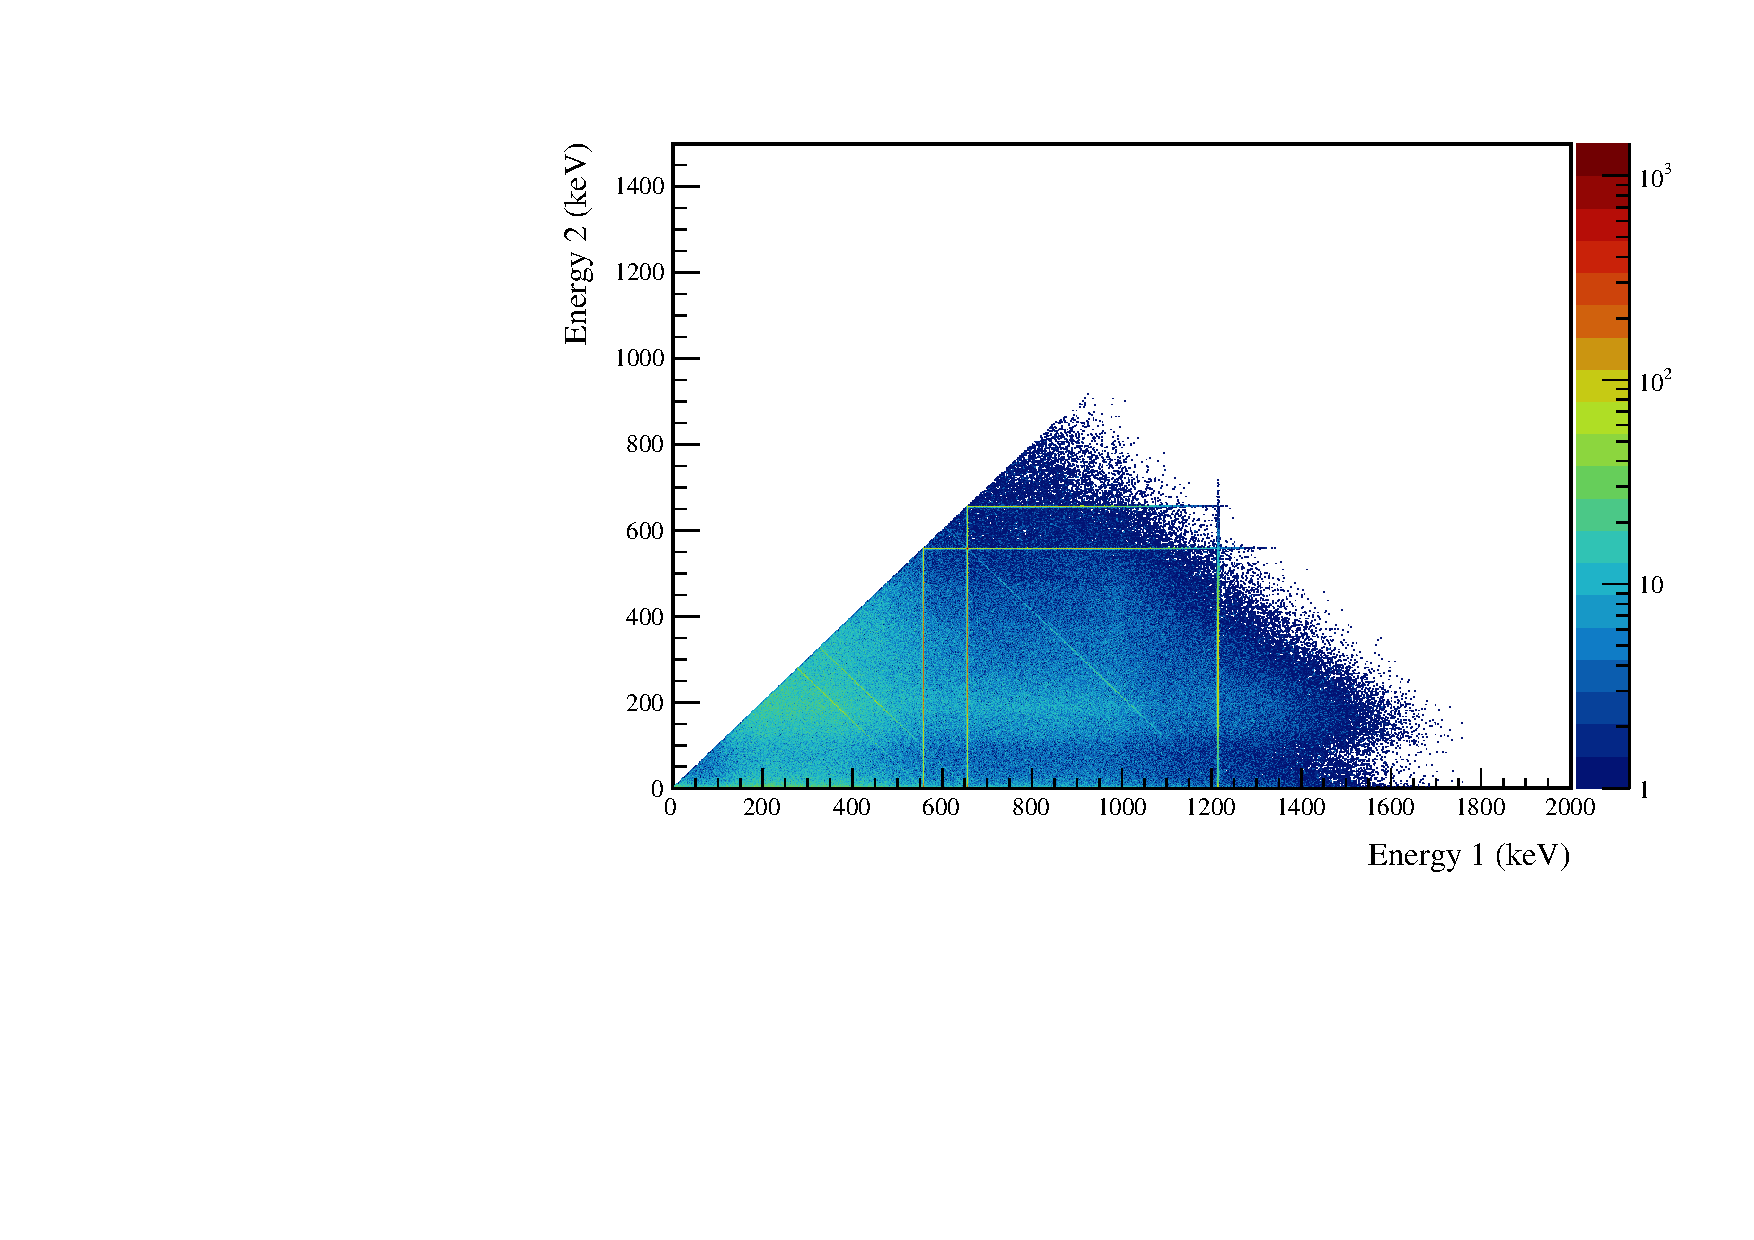
\includegraphics[width=.8\linewidth]{ESsim_2vBB_ES2_2}
  \caption[Simulation of \tnbb\ to \SP{2}{+}{2}]{
    Simulated multiplicity 2 energy spectrum of the \tnbb\ to \SP{2}{+}{2} decay mode}
\end{figure}

\subsection{559 keV peak}
\allmodeplots{2vBB_ES2_2_559}{\tnbb\ to \SP{2}{+}{2}}{559~keV peak}
\subsection{657 keV peak}
\allmodeplots{2vBB_ES2_2_657}{\tnbb\ to \SP{2}{+}{2}}{657~keV peak}
\subsection{1216 keV peak}
\allmodeplots{2vBB_ES2_2_1216}{\tnbb\ to \SP{2}{+}{2}}{1216~keV peak}



\section{\znbb\ to \SP{0}{+}{1}}
Note that both the 559~and 563~keV peaks will be shown together since they use the same sets of cuts.
\begin{figure}[!htb]
  \centering
  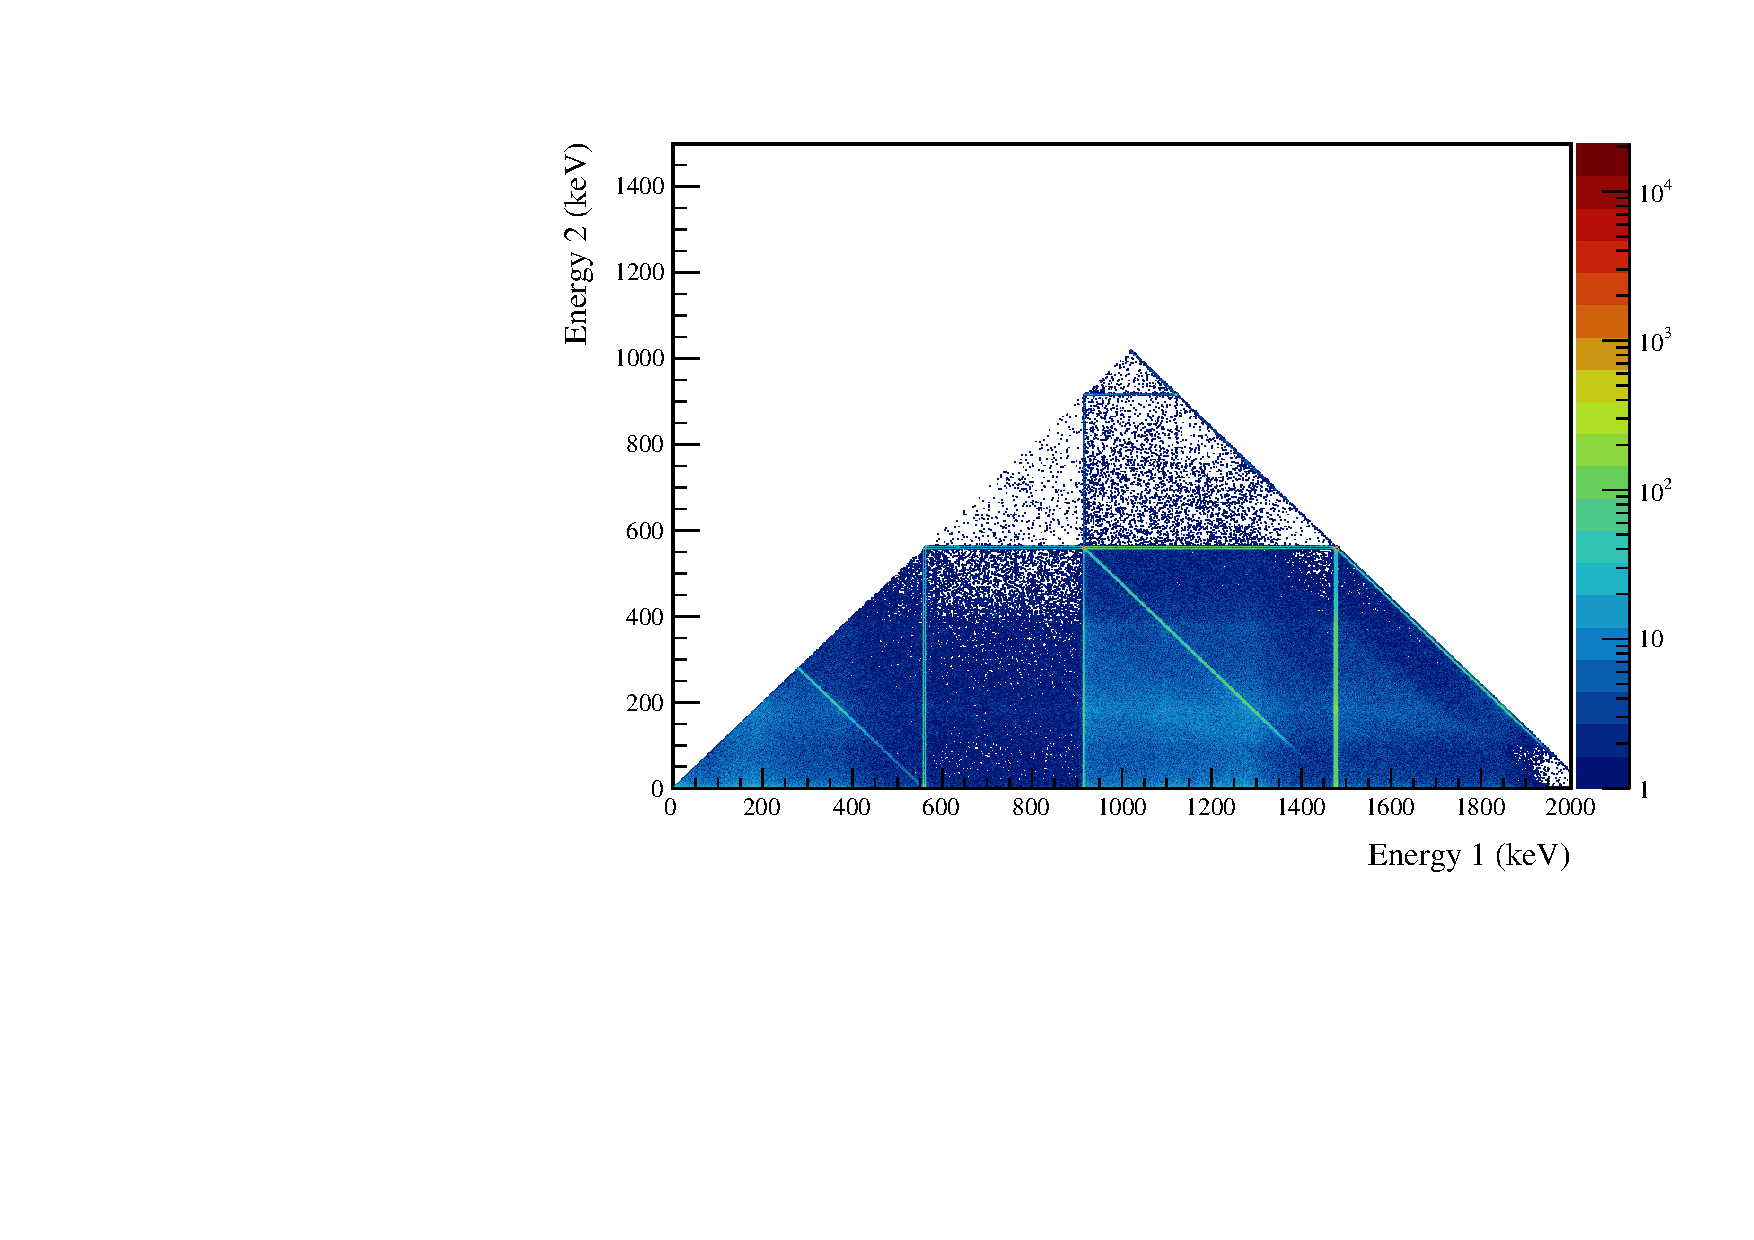
\includegraphics[width=.8\linewidth]{ESsim_0vBB_ES0_1}
  \caption[Simulation of \znbb\ to \SP{0}{+}{1}]{
    Simulated multiplicity 2 energy spectrum of the \znbb\ to \SP{0}{+}{1} decay mode}
\end{figure}

\allmodeplots{0vBB_ES0_1}{\znbb\ to \SP{0}{+}{1}}{559~and 563~keV peaks}

\section{\znbb\ to \SP{2}{+}{1}}
\begin{figure}[!htb]
  \centering
  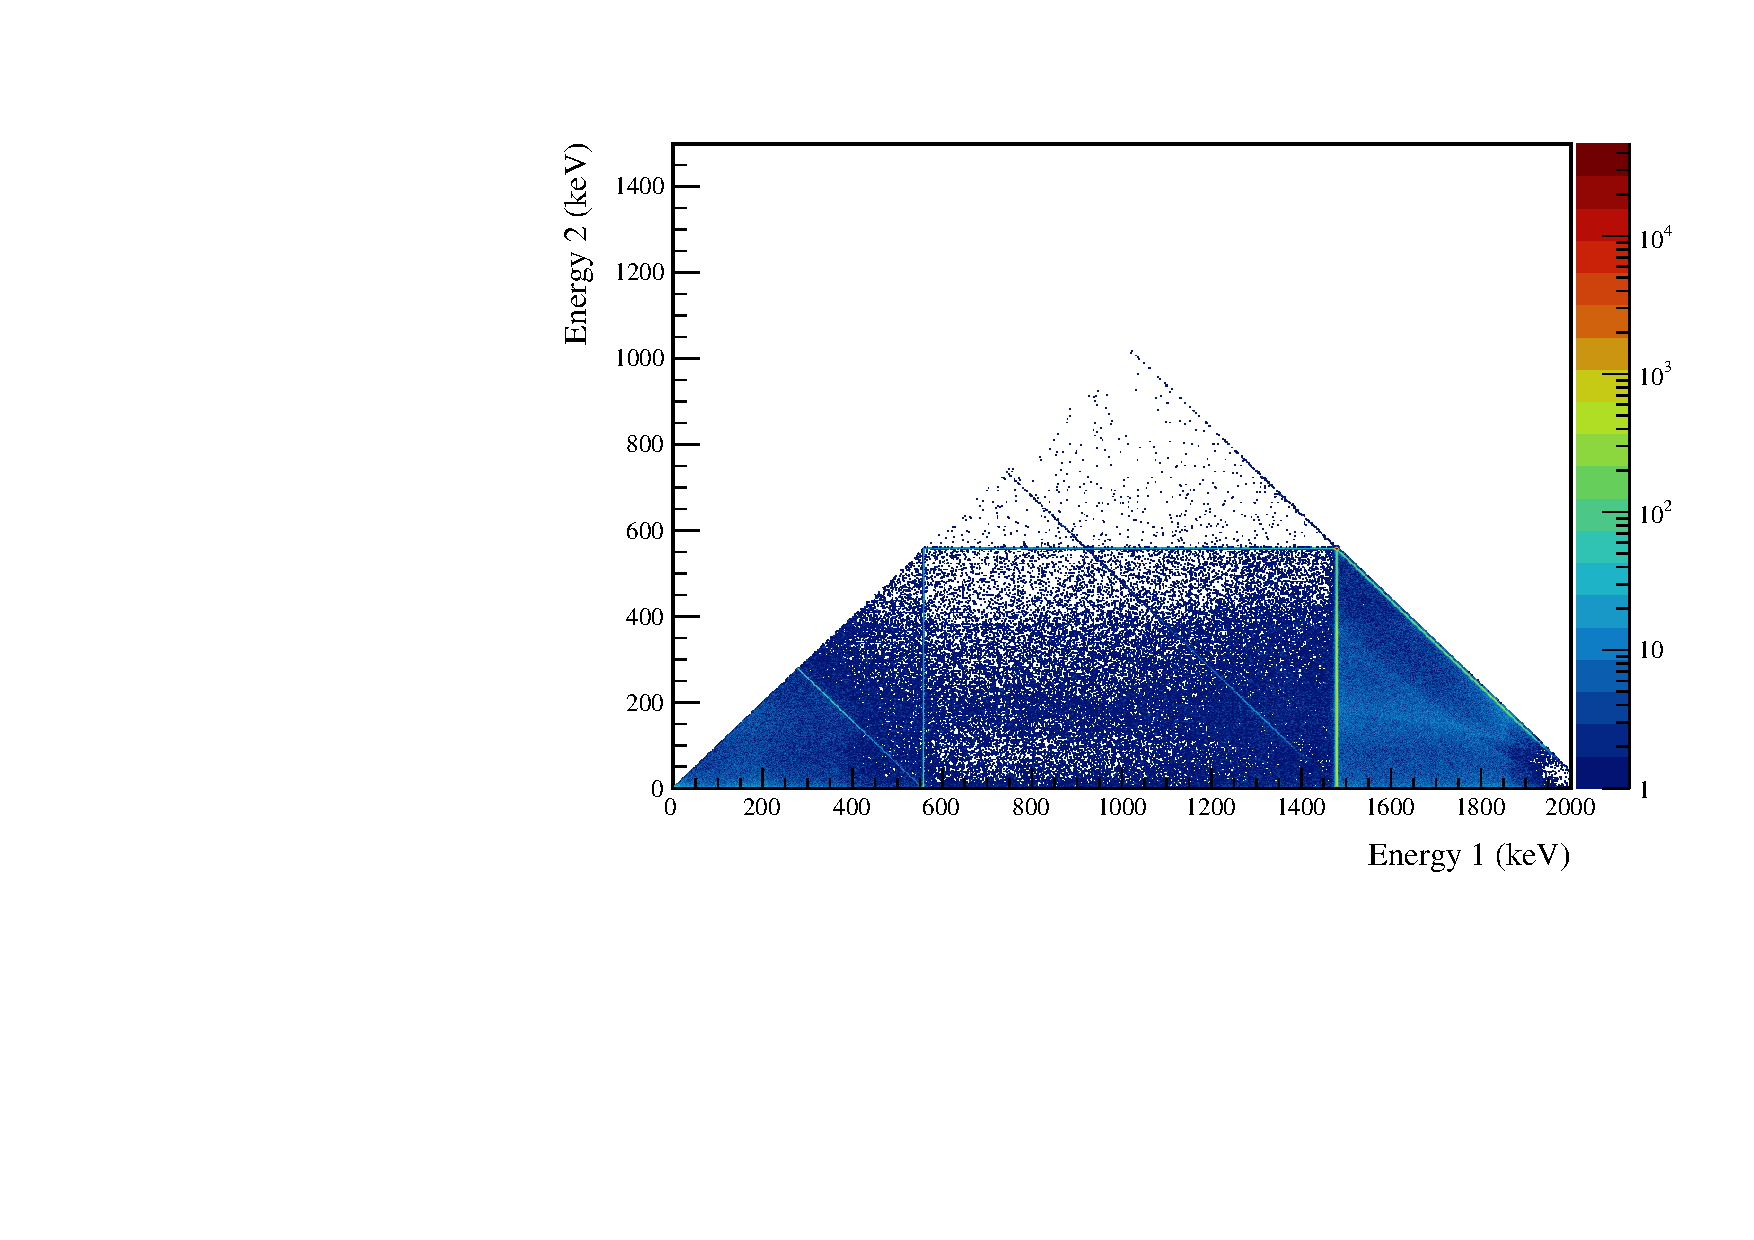
\includegraphics[width=.8\linewidth]{ESsim_0vBB_ES2_1}
  \caption[Simulation of \znbb\ to \SP{2}{+}{1}]{
    Simulated multiplicity 2 energy spectrum of the \znbb\ to \SP{2}{+}{1} decay mode}
\end{figure}

\allmodeplots{0vBB_ES2_1}{\znbb\ to \SP{2}{+}{1}}{559~keV peak}

\section{\znbb\ to \SP{2}{+}{2}}
\begin{figure}[!htb]
  \centering
  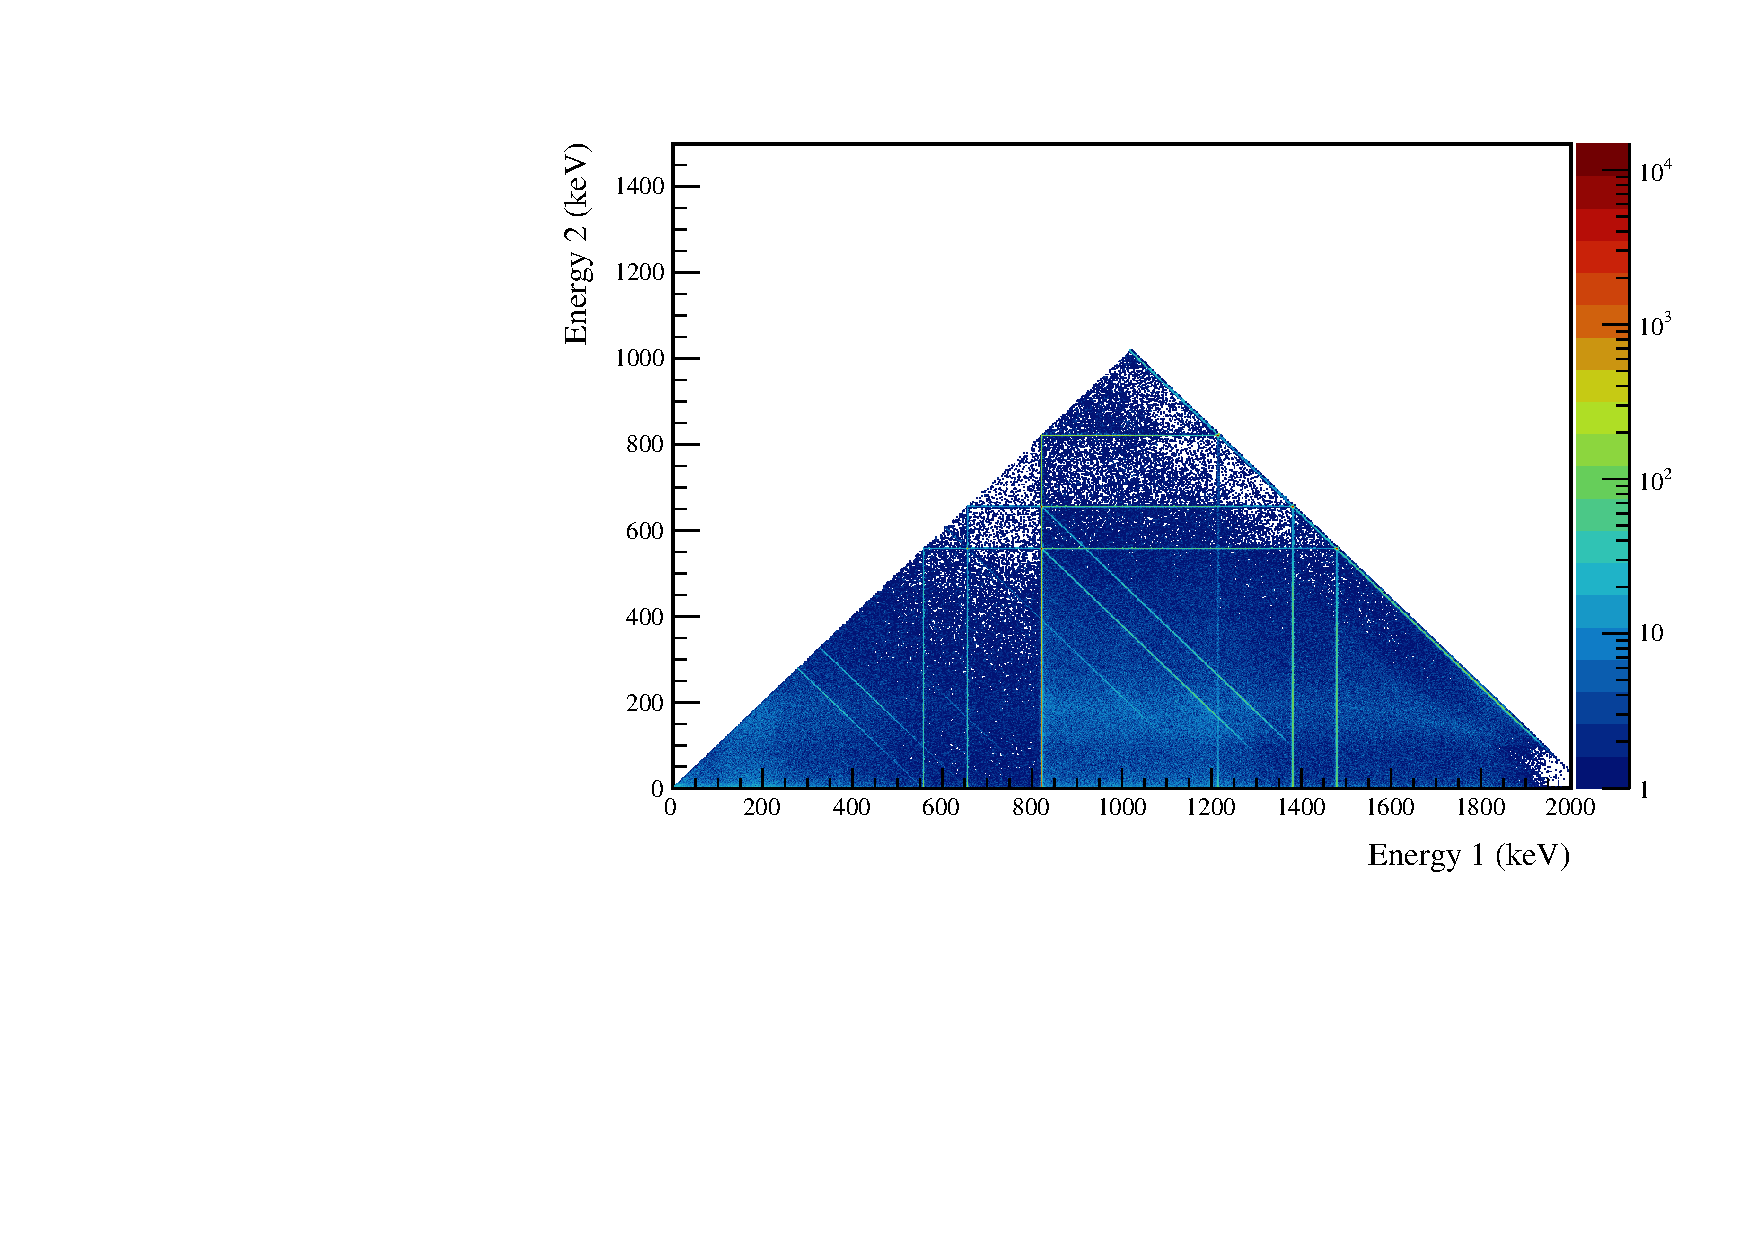
\includegraphics[width=.8\linewidth]{ESsim_0vBB_ES2_2}
  \caption[Simulation of \znbb\ to \SP{2}{+}{2}]{
    Simulated multiplicity 2 energy spectrum of the \znbb\ to \SP{2}{+}{2} decay mode}
\end{figure}

\subsection{559 keV peak}
\allmodeplots{0vBB_ES2_2_559}{\znbb\ to \SP{2}{+}{2}}{559~keV peak}
\subsection{657 keV peak}
\allmodeplots{0vBB_ES2_2_657}{\znbb\ to \SP{2}{+}{2}}{657~keV peak}
\subsection{1216 keV peak}
\allmodeplots{0vBB_ES2_2_1216}{\znbb\ to \SP{2}{+}{2}}{1216~keV peak}


\end{document}